\documentclass{beamer} % Use handout to get rid of repeated slides
\usetheme{AnnArbor}
\usecolortheme{default}
\usefonttheme{professionalfonts}
\usepackage{mathpazo}
 \usepackage{cancel}
\usepackage{listings}
\usepackage{xcolor}

% Define colors
\definecolor{myred}{RGB}{163,0,0}
\definecolor{ttcolor}{RGB}{0,0,1}%{RGB}{163,0,0}
\definecolor{mygray}{RGB}{248,249,250} 
\definecolor{mygreen1}{RGB}{0,96,0}
\definecolor{mygreen2}{RGB}{229,239,229}
\definecolor{aristotelgreen}{HTML}{008A44}
\definecolor{aristotelred}{HTML}{9E0101}
\definecolor{aristotelgrey}{HTML}{2E2E2E}
\definecolor{aristoteldarkred}{HTML}{500101}
\definecolor{aristotelorange}{HTML}{FF8C00}

\setbeamertemplate{theorem}[ams style]
\setbeamertemplate{theorems}[numbered]

\usepackage{etoolbox}

\undef{\definition}
\theoremstyle{definition}
\newtheorem{definition}{\translate{Definition}}
\hypersetup{
	colorlinks=true,
	linkcolor=aristotelorange,   % color for normal internal links
	citecolor=aristotelgreen,   % color for citation links
	urlcolor=aristotelgreen      % color for external links
}

\setbeamercolor{palette primary}{bg=aristotelred, fg=white}
\setbeamercolor{palette secondary}{bg=aristoteldarkred, fg=white}
\setbeamercolor{palette tertiary}{bg=black, fg=white} 

\setbeamercolor{title}{fg=white, bg=aristotelred} % Title text color
\setbeamercolor{subtitle}{fg=white, bg=aristotelred} % Subtitle text color
\setbeamercolor{background canvas}{bg=aristotelgrey} % Background for content canvas
\setbeamercolor{normal text}{fg=white} % Normal text color
\setbeamercolor{titlegraphic}{bg=mygray} % Background color for title graphic area
\setbeamercolor{frametitle}{fg=white, bg=aristoteldarkred}

% Change color of numbered circles in the table of contents
\setbeamercolor{section number projected}{bg=white, fg=black}
\setbeamercolor{subsection number projected}{bg=aristotelred, fg=aristotelgrey}
\setbeamercolor{subsection number projected}{bg=aristotelorange, fg=white}

\setbeamercolor{block title}{fg=white,bg=mygreen1}
\setbeamercolor{block body}{fg=black,bg=mygreen2}


\lstdefinestyle{rstyle}%
{language=[LaTeX]TeX,
	basicstyle=\footnotesize\ttfamily,
	backgroundcolor = \color{mygray},
	commentstyle=\slshape\color{green!50!black},
	keywordstyle=\color{blue},
	identifierstyle=\color{blue},
	stringstyle=\color{orange},
	%escapechar=\#,
	rulecolor = \color{mygray}, 
	showstringspaces = false,
	showtabs = false,
	tabsize = 2,
	emphstyle=\color{red},
	frame = single} 

\begin{document}
	\title[Paper presentation]{Presentation of a paper:}
	\subtitle[subtitle?]{A Test for Relative Efficiency and Application to Indian Agriculture \\ Lawrence J. Lau \& Pan A. Yotopoulos (1971) }
	\author[Riste Petrov]{Riste Petrov \\ \href{mailto:riste@uni-sofia.bg}{riste@uni-sofia.bg}}
	\institute[AEEM - FEBA]{AEEM - FEBA - Sofia University St. Kliment Ohridski - coh. 2026/27}
	\titlegraphic{\includegraphics[scale=0.5]{/home/anonymous/Documents/Mega/ЦЕЛ/Master/1Courses/SU ENG White horizontal.pdf}}
	\date{\today}
	
	\begin{frame}[fragile]
		\titlepage
	\end{frame}
	
	\begin{frame}[fragile]
		\frametitle{Contents}
		\tableofcontents[]
	\end{frame}
	
	\section{Introduction}
	\subsection{Authors}
	\begin{frame}[fragile]
		\frametitle{Background of the authors}
		\framesubtitle{Academic}
		\textbf{Lawrence J. Lau} \\
			is a Hong Kong economist, former Chancellor of Chinese University of Hong Kong \& economics professor at Stanford. He has a B.S. in physics \& economics from Stanford, M.A. \& Ph.D. from Berkeley. In 1966 after graduating the M.A. he was joined the Stanford Faculty, after the paper in 1976 he became a Professor of Economics in 1976.\\
			
			\vspace{1em}
			\textbf{Pan A. Yotopoulos}\\
			was a Greek Economist in the field of economic development and agricultural economics, economic demography, international trade, production and consumption theory. He joined Stanford as a Associate Professor in 1968.
	\end{frame}
	
	\subsection{Common connection}
	\begin{frame}[fragile]
		\frametitle{Connection of the paper with my experience}
		\framesubtitle{My bachelor degree thesis}
		\textbf{Analysis of Profitability in Small Individual Grape Producers in North Macedonia} — {\tiny Published in Macedonian in the UGD Economics Faculty Yearbook 2025 (Vol 27 No.1) }\\
		\vspace{.5em}
		Using a 4-plantation sample, I collected all economic inputs and outputs to run scenario analyses and evaluate their effects on:
		\begin{itemize}
			\item H0 - Lack of Capital $\rightarrow$ higher operating costs $\rightarrow$ financial unsustainability
			\item H1 - Short - term subsidies $\rightarrow$ lower product quality $\rightarrow$ spreading of Phytopathogens
			\item H2 - Small producers lack economies of scale for sustainable practices
		\end{itemize}
		\textbf{Quick conclusion}\\
		\begin{small}
			The government's subsidy policy aims to preserve the status quo and protect political capital. 
		\end{small}
	\end{frame}
	
	\begin{frame}[fragile]
		\frametitle{North Macedonia Grape \& India}
		\framesubtitle{Investment management $\cancel{\rightarrow}$ Micro 3}
		\begin{minipage}[t]{0.48\textwidth} 
			\centering \textbf{Grape}\\[0.5em] 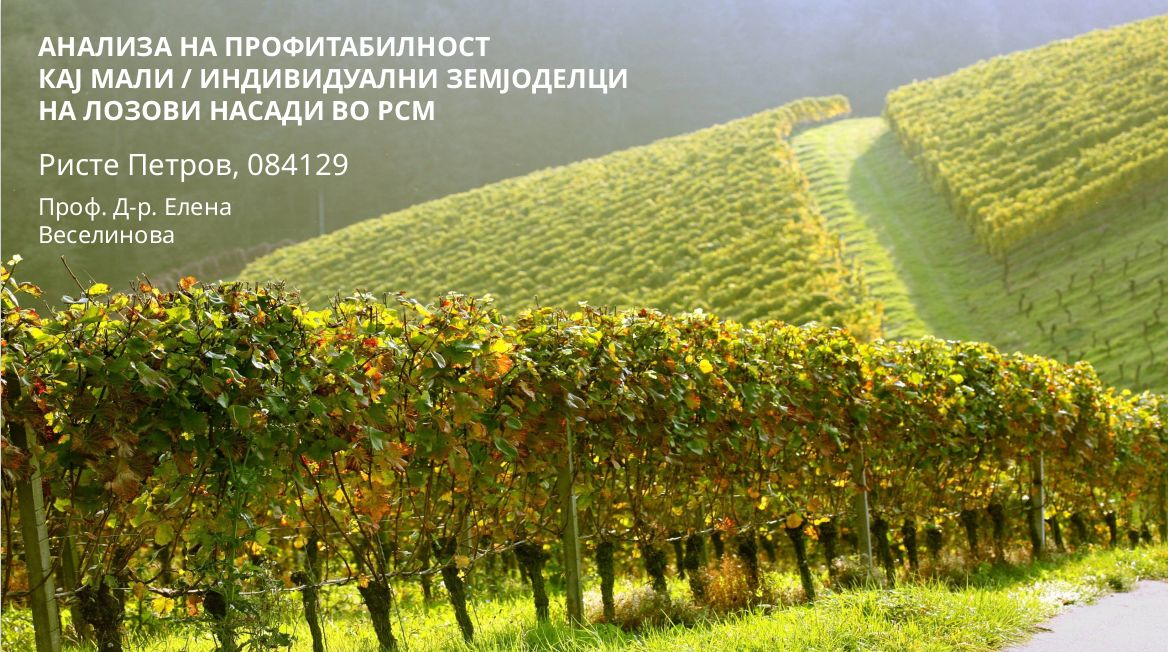
\includegraphics[width=\linewidth]{wine.jpeg} 
		\end{minipage}\hfill 
		\begin{minipage}[t]{0.48\textwidth} 
			\centering \textbf{India}\\[0.5em] 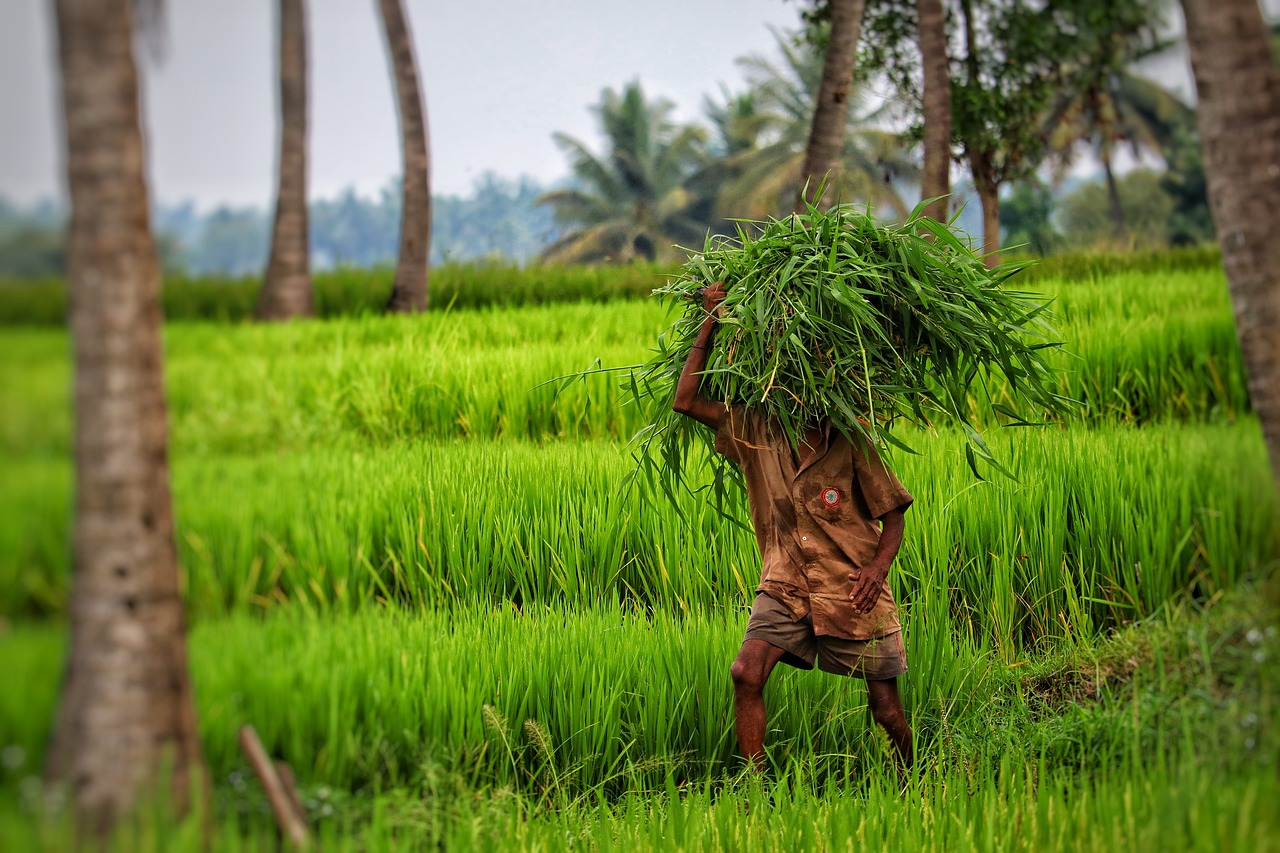
\includegraphics[width=\linewidth]{india.jpg} 
		\end{minipage} 
	\end{frame}
	
	\section{Research}
	\begin{frame}[fragile]
		\frametitle{The crucial theory}
		\framesubtitle{Back to Micro 3}
		Starting of with the most basic formula:
		$$ V^1 = A^1F(X^1); \qquad V^2 = A^2F(X^2) $$
		\begin{center}
			Technical efficiency if $A^1 > A^2$ produces better profits.\\
			 {\tiny Same conclusion was derived with the improvement in the process in the North Macedonian small sample case - Cost reduction}
		\end{center}
		After all the derivation the authors present the "Unit-Output-Price" \& profit function.
		$$ P = \frac{P'}{p} = F(X_1,\hdots, X_m; Z_1, \hdots Z_n) - \sum_{i=1}^{m} c_iX_i $$ 
		$$ X_i^{*} = f_i(c,Z), \quad i = 1, \hdots, m$$
		
		
	\end{frame}
	
	\begin{frame}[fragile]
		\frametitle{The crucial theory 2 }
		\framesubtitle{Continuation from the first theory slide}
		Continuation from the last slide:
		$$ \prod = p\left[F(X_1^*, \hdots , X_m^*, Z_1 \hdots, Z_n - \sum_{i=1}^{m} c_iX_i^*  \right] = G(p,c_1', \hdots, c_m';Z_1, \hdots, Z_n) $$
		So the final UOP profit function is:
		$$ \prod\nolimits^* = \frac{\prod}{p} = G^*(c_1, \hdots, c_m; Z_1, \hdots, Z_n)$$
		Using Shepar-Uzawa-McFadden Lemma equation:
		$$ V^* = \prod\nolimits^*(c,Z) - \sum_{i=1}^{m} \frac{\delta \prod\nolimits^*(c,Z)}{\delta c_i} \cdot c_i$$
		
	\end{frame}
	
	\begin{frame}[fragile]
		\frametitle{The crucial theory 3 }
		\framesubtitle{Cobb–Douglas derivation}
		After all the derivation we get to:
		\begin{equation*}
			\ln \prod\nolimits_a^1 = \ln A^1_* + \sum_{j=1}^n \alpha_j^* \ln c_j^1 + \sum_{j=1}^n \beta_j^* \ln Z_j^1
		\end{equation*}
		\begin{equation*}
			\ln \prod\nolimits_a^2 = \ln A^1_* +  \ln \frac{A_*^2}{A_*^1} + \sum_{j=1}^n \alpha_j^* \ln c_j^2 + \sum_{j=1}^n \beta_j^* \ln Z_j^2
		\end{equation*}
		Where:
		\begin{itemize}
			\item $\prod\nolimits_a$ - the profit/production aggregate
			\item $A*$ - the productivity
			\item $\ln \frac{A_*^2}{A_*^1}$ - change in productivity
			\item $c_j$ - conventional input
			\item $Z_j$ - quasi-fixed exogenous factor $Z_j$
		\end{itemize}
	\end{frame}
	
	\begin{frame}[fragile]
		\frametitle{Empirical Application}
		\framesubtitle{Empirical Cobb–Douglas applied}
		
		\begin{equation*}
			\ln \prod\nolimits_a^1 = \ln A_*^1 + \alpha_1^* \ln w + \beta_1^* \ln K + \beta_2^* \ln T
		\end{equation*}
		\begin{equation*}
			\ln \prod\nolimits_a^2 = \ln A_*^1 + \ln \frac{A_*^2}{A_*^1} + \alpha_1^* \ln w + \beta_1^* \ln K + \beta_2^* \ln T
		\end{equation*}
		Final estimation:
		\begin{equation*}
			\ln \prod = \alpha + S + \sum_{i=1}^{4} \delta_i^* D_i + \alpha^*_1 \ln w' + \beta^*_1 \ln K + \beta^*_3 \ln T
		\end{equation*}
		
		
		
	\end{frame}
	
	\begin{frame}[fragile]
		\frametitle{Results}
		\framesubtitle{From the Indian Sample Case}
		\begin{center}
			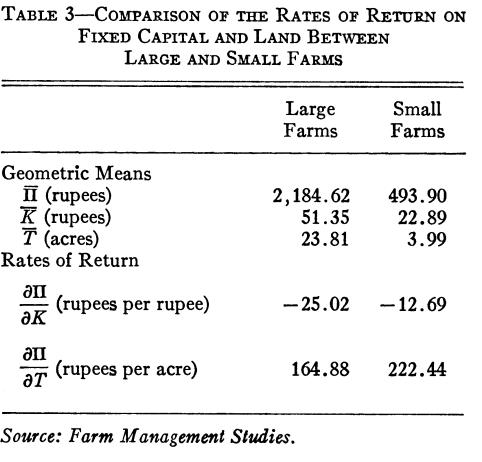
\includegraphics[width=0.55\textwidth,height=0.7\textheight]{conclusion.png}
		\end{center}
	\end{frame}
	
	
	
	\section{Q\&A}
	\begin{frame}[fragile]
		\frametitle{Ending remarks}
		\begin{center}
			I am delighted for your attention.\\
			\vspace{1em}
			Q \& A?
		\end{center}
	\end{frame}
	
\end{document}